\section{Билет 29. Понятие области с границей $C^2$. Потенциал просто слоя. Его свойства. Непрерывность в $\R^3$}
% Затехал: Цветкова Ольга
\begin{definition}
{\bf Область с границей Г класса $C^2$} - ограниченная область ($\Omega \subset \R^3$), удовлетворяющая условиям :
\begin{itemize}
\item $\forall x^0 \in \text{Г} \Exists \text{ декартова с.к.} (\xi_1, \xi_2, \xi_3) \text{ с началом в } x^0 \text{ и функция } F_{x^0}(\xi'), \text{ где } \xi'~=~(\xi_1, \xi_2),\\ |\xi'|~\leqslant~r \ \text{ т.что }$
	\begin{itemize}
	\item $F_{x^0}(\xi') \in C^2(|\xi'| \leqslant r);\ F_{x^0}(0,0) = 0,\;\frac{\partial F_x}{\partial \xi_i}(0,0)=0,\ i=1,2  $
	\item Множество $\sum_{x^0} = \{x:\ \xi_3 = F_{x^0}(\xi'), |\xi'|\leqslant r\} \subset \text{Г}$
	\item Множество $\text{U}_{x^0}^{-}= \{x:\ F_{x^0}(\xi') - h < \xi_3 <F_{x^0}(\xi'),\ |\xi'|< r \} \subset \Omega$
	\item Множество $\text{U}_{x^0}^{+}= \{x:\ F_{x^0}(\xi') < \xi_3 <F_{x^0}(\xi')+h,\ |\xi'|< r \} \text{ не пересекается с } \Omega$
	\end{itemize}
	\item $F_{x^0}(\xi') \in C^2(|\xi'| \leqslant r) \Rightarrow \abs{\pd{F_x}{\xi_i}} \leqslant M_1; \abs{\cfrac{\partial^2F_x}{\partial\xi_i\partial\xi_j}} \leqslant M_2, |\xi'|\leqslant r$
	\item Постоянные $r > 0,\ h>0 \text{ и } M_1, M_2$ можно выбрать не зависящими от $x^0 \in \text{Г}$ и от с.к. $\xi$
\end{itemize}
\end{definition}
\begin{definition}
Указанную с.к. и окрестность $U_{x^0} = \text{U}_{x^0}^{-} \cup \text{U}_{x^0}^{+}$ назовем {\bf подходящим для $X^0$}, а $\xi'$ - {\bf локальными координатами} на куске $\sum_{x^0} \text{ границы } \text{Г}.$
\end{definition}

\begin{definition}
Неограниченная область называется {\bf внешней областью с границей Г$\in C^2$}, если  $\R^3 \backslash \bar{\Omega}$ есть ограниченная область с границей $\in C^2.$
\end{definition}

\begin{definition}
Пусть $\Omega \subset \R^3 $- область с границей Г класса $C^2$. Функция  вида $V^{(0)}(x) = \int_{\text{Г}} \cfrac{\mu(y)}{|x-y|} dS_y$ называется {\bf потенциалом простого слоя}.
\end{definition}

\begin{theorem}
 Пусть $\mu(x) \in \C(\text{Г})$. Тогда:
 	\begin{enumerate}
 	\item $V^0(x) \in C(\R^3)$
 	\item $V^0(x) \text{ гармоническая в } \R^3 \backslash$Г
 	\item $V^0(x) = O\big( \cfrac1x \big)$ при $x \rightarrow \infty$
 	\end{enumerate}
\end{theorem}
\begin{proof}

\begin{enumerate}
\item[2.] Пусть $x^1 \in \R^3 \backslash \text{Г},\ \delta_1 = \text{dist}\{x^1,\text{Г}\}> 0$

\begin{center}
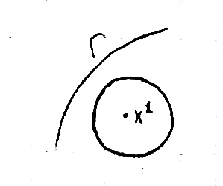
\includegraphics[scale = 0.7]{29_1_new}
\end{center}

Возьмем шар $B(x^1, \cfrac{\delta_1}{2}) = \{ x \in \R^3 : |x - x^1| < \cfrac{\delta_1}{2}\}$. Тогда расстояние от произвольной точки $x \in \overline{B(x^1, \cfrac{\delta_1}{2})} \text{ до } \forall y \in \text{Г} \text{ не меньше } \cfrac{\delta_1}{2} : |x-y| \geqslant |x^1-y|-|x-x^1| \geqslant \delta_1 - \cfrac{\delta_1}{2} = \cfrac{\delta_1}{2} $

Поэтому $\cfrac{1}{|x-y|} \in C^\infty(\underbrace{\overline{B(x^1, \cfrac{\delta_1}{2})}}_x \times \underbrace{\text{Г}}_y)\Rightarrow \mathcal{D}_x^\alpha\cfrac{1}{|x-y|} \in C(\overline{B(x^1, \cfrac{\delta_1}{2})} \times \text{Г})$

По теореме о дифференцировании интеграла по параметру (формулировка в билете 5) имеем
\[
\mathcal{D}_x^\alpha V^{(0)}(x) = \int_{\text{Г}} \mathcal{D}_x^\alpha\cfrac{\mu(y)}{|x-y|} dS_y \in C(\overline{B(x^1, \cfrac{\delta_1}{2})} \times \text{Г})\Forall\alpha\text{-мультииндекса}
\]
В частности, $\bigtriangleup_x V^{(0)}(x) = \int_{\text{Г}} \bigtriangleup_x(\cfrac{1}{|x-y|})\mu(y) dS_y = 0$, что и требовалось.
\item[1.] Если $x \in \text{Г, то } \cfrac{1}{|x-y|}$ - полярное ядро, следовательно, интегральный оператор с полярным ядром переводит непрерывную функцию $\mu(y)$ в непрерывную $\Rightarrow V^{(0)}(x) \in C(\text{Г})$.

Мы уже доказали, что $V^{(0)}(x) \in C(\R^3 \backslash \text{Г}) \Rightarrow$ осталось показать непрерывность в областях $\Omega$ следующего вида:

\begin{center}
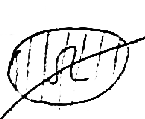
\includegraphics[scale = 0.6]{29_2_new}
\end{center}



Построим для этого последовательность функций, равномерно сходящихся к $V^{(0)}(x)$:

Пусть $\biggl(\cfrac{1}{|x-y|}\biggr)_\delta - \delta\text{-срезка функции } \cfrac{1}{|x-y|}: $
\[
\biggl(\cfrac{1}{|x-y|}\biggr)_\delta=\begin{cases}
\cfrac{1}{|x-y|},&\text{если $|x-y|\geqslant \delta$;}\\
\cfrac{1}{\delta},&\text{если $|x-y|<\delta$.}
\end{cases}
\]
$V^{(0)}_\delta(x) = \int_{\text{Г}} \biggl(\cfrac{1}{|x-y|}\biggr)_\delta\mu(y) dS_y \in C(\overline{\Omega})$

Будем выбирать $0 < \delta < \cfrac{d}{2} (d - \text{из свойств области с границей класса }C^2) - \text{ такое число, что }\forall x^0 \in \text{Г} \rightarrow B(x^0, d) \subset U_{x^0}$
\[
\biggl| V^{(0)}(x) - V_\delta^{(0)}(x) \biggr| = \biggl| \int_{\text{Г}} \Biggl(\cfrac{1}{|x-y|} - \biggl(\cfrac{1}{|x-y|}\biggr)_\delta\Biggr)\mu(y) dS_y \biggr|
\]

Если $x : |x-y| \geqslant \delta$, то $ \Biggl(\cfrac{1}{|x-y|} - \biggl(\cfrac{1}{|x-y|}\biggr)_\delta\Biggr)= 0 $

В противном случае она равна $\biggl|\int_\text{Г}\underbrace{(\cfrac{1}{|x-y|} - \cfrac{1}{\delta})}_{>0}\underbrace{\mu(y)}_{|\mu(y)| \leqslant  ||\mu||_{C(\text{Г})} = C} dS_y \biggr| \geqslant C\int\limits_{\substack{y \in \text{Г} \\ |x-y|<\delta}}\cfrac{dS_y}{|x-y|}$


Нам осталось оценить интеграл $\int\limits_{\substack{y \in \text{Г} \\ |x-y|<\delta}}\cfrac{dS_y}{|x-y|}$

\begin{center}
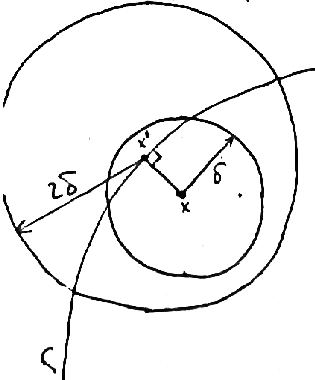
\includegraphics[scale = 0.25]{29_3_new}
\end{center}

Пусть $x^* = \pi_\text{Г}(x)$. Построим $B(x,\delta)$ и $B(x^*, 2\delta)$.

Ясно, что т.к. $|x - x^*| < \delta \Rightarrow B(x, \delta) \subset B(x^*, 2\delta)$.

Увеличивая область интегрирования, запишем:


\[
\int_{\substack{y \in \text{Г} \\ |x-y|<\delta}}\cfrac{dS_y}{|x-y|} \leqslant \int\limits_{\substack{y \in \text{Г} \\ |x^*-y|<2\delta}}\cfrac{dS_y}{|x^*-y|}
\]
По определению числа d имеем $B(x^*, 2\delta \subset U_{x^*})$. 
\begin{center}
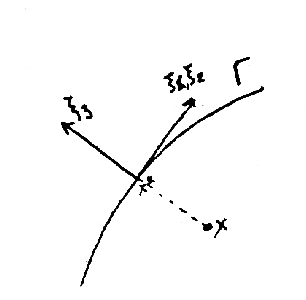
\includegraphics[width=0.2\linewidth]{29_4_new} 
\end{center}

Свяжем с $x^*$ локальную систему координат и функцию $F_{x^*} (\xi_1, \xi_2)$


Т.к. $y \in \text{Г}, y = (\xi_1, \xi_2, F_{x^*}(\xi_1, \xi_2))$

Т.к. $x^* = \pi_\text{Г}(x)$, точка x имеет ненулевую компоненту только по $\xi_3\ :\ x = (0,0,x_3)$


Оценки: $|x-y|^2 = \xi_1^2 + \xi_2^2 + (x_3 - F_{x^*}(\xi_1, \xi_2))^2 \leqslant \xi_1^2 + \xi_2^2$ \\ 
$|x^*-y|^2 = \xi_1^2 + \xi_2^2 + (F_{x^*}(\xi_1, \xi_2))^2 \leqslant \xi_1^2 + \xi_2^2 \Rightarrow$ расширяем область интегрирования до $\sqrt{\xi_1^2 + \xi_2^2} < 2\delta$
\[
\biggl| V^{(0)}(x) - V_\delta^{(0)}(x) \biggr| \geqslant C \int\limits_{\sqrt{\xi_1^2 + \xi_2^2} < 2\delta} \cfrac{\sqrt{1 + (\pd{F_{x^*}}{\xi_1}(\xi_1, \xi_2))^2 +  (\pd{F_{x^*}}{\xi_2}(\xi_1, \xi_2))^2}}{\sqrt{\xi_1^2 + \xi_2^2}}d\xi_1d\xi_2 \leq
\] 
\[C \sqrt{1 + 2M_1^2} \int\limits_{\sqrt{\xi_1^2 + \xi_2^2} < 2\delta} \cfrac{d\xi_1d\xi_2}{\sqrt{\xi_1^2 + \xi_2^2}}
\]

В полярной системе координат $\bigl(\begin{smallmatrix}
\xi_1 \\ \xi_2
\end{smallmatrix}\bigr) = r \bigl(\begin{smallmatrix}
\cos \varphi \\ \sin \varphi
\end{smallmatrix}\bigr)$ последний интеграл примет вид $\int\limits_{0}^{2\pi}d\varphi \int\limits_{0}^{2\delta}\cfrac{rdr}{r} = 4\pi\delta \rightarrow 0 \text{ при } \delta \rightarrow 0.$

Итак, $\underbrace{V_\delta^{(0)}(x)}_{\in C(\overline{\Omega})}\rightrightarrows_{\delta \rightarrow 0} V^{(0)}(x) \Rightarrow V^{(0)}(x) \in C(\overline{\Omega})\Rightarrow V^{(0)}(x) \in C(\R^3)$.

\item[3.] $\mu(x) \in \text{Г}\Rightarrow |\mu(x)|\leqslant ||\mu||_{\text{Г}} = C \Forall x \in \text{Г}$

Возьмем сферу радиуса R такую, что Г лежит внутри этой сферы. Тогда $\forall y \in \text{Г} \rightarrow |y| \leqslant R.$

При $x \rightarrow \infty\  \rightarrow |x|\geqslant 2R\ \Rightarrow y \leqslant \cfrac{|x|}{2} \ \Rightarrow |V^0(x)| \leqslant \int_{\text{Г}}\cfrac{|\mu(y)|}{|x-y|}dS_y \leqslant \cfrac{2C}{|x|}\underbrace{\int_\text{Г}dS_y}_{\mathbf{\vec C}} \Rightarrow V^0(x) = O(\cfrac{1}{|x|}) \text{ при } x \rightarrow \infty.$
\end{enumerate}
\end{proof}